\subsection{Experiment Three}\label[subsec]{subsec:exp_three}

The third experiment investigated \cref{RQ:RQ3,RQ:RQ4}, by taking a look at the per-core performance. In this experiment only IPG and the Clamp was used to conduct measurements. This experiment will explore what benefit macrobenchmarks gain from additional allocated cores, by executing PCM and 3DM on an increasing number of cores. Before this is done, an analysis on the per-core performance of both CPUs will be conducted, where the single-core benchmarks introduced in \cref{subsec:test_cases} will be used. This allowed a comparison between the energy consumption of the P- and E-cores on DUT 2 and the P-cores on DUT 1. When performing measurements, the limit of $1.000$ measurements set in \cref{subsec:exp_two} is still used.

%The benchmark used in this experiment was the single-core benchmarks introduced in \cref{subsec:test_cases}, by running each benchmark on one core at a time, while measuring the energy consumption using IPG and Clamp. This will show how the performance is between P- and E-cores, and how the performance is between cores with the same specifications.

\paragraph{Per-Core Initial Measurements:} An initial $250$ measurements were made for each benchmark on each core. Then Cochran's formula was calculated to determine if more measurements were required. Results from Cochran's can be found in \cref{app:exp_three_coch}.

%The first measurements were made, will be in order to compare the per-core performance, where $250$ measurements will be made for each benchmark on each core. After $250$ measurements, more measurements were made where it was required, as can be found in \cref{app:exp_three_coch}, with an upper limit of $1000$ measurements.

\begin{table}[H]
    \centering
    \begin{tabular}{|| c | c | c | c ||}
    \hline
    \multicolumn{4}{||c||}{SN measurements on DUT 2} \\ [0.5ex] \hline\hline
    Metric & E-core & P-core & Difference \\\hline
    Execution time & $58.96$ s & $13.96$ s & $-76.32$\% \\
    Energy & $336.88$ j & $99.53$ j & $-70.45$\% \\
    DEC & $253.85$ j & $16.26$ j & $-93.59$\% \\
    DEC per second & $0.53$ w & $1.88$ w & $+254.71$\% \\\hline
    \end{tabular}
    \caption{The average performance difference between P and E cores on DUT 2, SN}
    \label{tab:dut-2-exp-3-sn}
\end{table}


% DEC, E
%  - 249.81 + 255.66 + 254.87 + 255.08 = 253.85
% DEC, P
%  - 17.04 + 15.28 + 16.19 + 15.94 + 16.40 + 16.72 = 16.26

% diff = 93.59



% DEC PS, E
%  - 0.51 + 0.51 + 0.54 + 0.55 = 0.53
% DEC PS, P
%  - 1.87 + 1.88 + 1.87 + 1.89 + 1.85 + 1.90 = 1.88

% diff = 254.71


% DUR, E
%  - 59.03 + 58.92 + 58.97 + 58.92 = 58.96
% DUR, P
%  - 14 + 13.98 + 13.98 + 13.89 + 13.98 + 13.98 = 13.96

% diff = 76.32

% ENERGY, E
%  - 331.68 + 339.69 + 338.02 + 338.12 = 336.88
% ENERGY, P
%  - 100.45 + 99.42 + 99.20 + 99.23 + 99.24 + 99.68 = 99.53

% diff 70.45

\paragraph{Per-Core Results:} The results, presented here are based on DUT 2, where the results will be shown in tables, given the low deviation in the results. Boxplots for both DUTs can be found in \cref{app:exp_three}. For SN, as seen in \cref{tab:dut-2-exp-3-sn}, the run time was on average $76.26\%$ lower on the P-cores compared to the E-cores and The total DEC was on average $70.44\%$ lower on P cores, however the E cores had a $72.88\%$ lower energy consumption per second. %When comparing  P- and E-cores, the duration is on average is $76.26\%$ lower on P cores, the energy consumption is $70.44\%$ lower on P cores over the entire duration, while E cores has a $72.88\%$ lower energy consumption per second.
The largest difference between two cores of the same type was found on DUT 1 with benchmark NB, where the performance was $11.61\%$ worse on core 1 than core 6. The smallest difference was found on DUT 2, benchmark NB on a E core, where the energy consumption was $1.17\%$ higher on core $6$ than core $9$.

%When comparing cores of the same type, the largest difference between the best and worst performing core was found on DUT 2, with benchmark NB, 



% dut 1, NB: 11.61 2 and 7
% dut 1, SN: 2.5
% dut 2, NB: E:3.38, P: 1.17
% dut 2, SN: E: 1.26, P:2.35

\paragraph*{Macrobenchmark Initial Measurements:} An initial $30$ measurements were made for both 3DM and PCM on an increasing number of cores. The initial idea was to start at one core, which is done for 3DM for both DUTs and PCM on DUT 1. On DUT 2, PCM could not execute web browsing on a single core, and was unable to execute spreadsheet and photo editing. Because of this, DUT 2 will start at 2 cores. For DUT 1, web browsing was unable to execute, so this scenario is excluded for this DUT. $30$ measurements was chosen as the per-core experiment illustrated how $250$ was too much for DUT 2. The order of cores used in this experiment was done by using the cores with the lowest DEC found in \cref{app:exp_three}. The required measurements from the first $30$ according to Cochran's can be found in \cref{app:exp_three_coch_app}.

\begin{figure}[H]
    \centering

\begin{tikzpicture}
\pgfplotsset{
    every axis/.style={ymin=0},
    width=0.22\textwidth,
    height=0.25\textheight,
    xtick={1, 2, 3, 4, 5, 6, 7, 8, 9, 10},
    y axis style/.style={
    yticklabel style=#1,
    ylabel style=#1,
    y axis line style=#1,
    ytick style=#1}}
\begin{axis}[ scale only axis, ymin=0, ymax=170, xmin=1,xmax=10, axis y line*=left, xlabel=Number of Cores, ylabel=Duration (s), y axis style=green!75!black]
    \addplot[smooth, green!75!black, mark=o, draw] 
    coordinates 
    {
        (1,163.94299999999998)
        (2,107.274)
        (3,88.25800)
        (4,79.17)
        (5,73.277)
        (6,70.9025)
        (7,69.2505)
        (8,70.0790000)
        (9,66.7965000)
        (10,69.183500)
    };
\end{axis}
%
\begin{axis}[ scale only axis, ymin=0, ymax=1800, xmin=1,xmax=10, axis y line*=right, axis x line=none, ylabel=DEC (j), y axis style=blue]%
    \addplot[smooth, blue, mark=x] 
    coordinates 
    {
        (1,1127.21859)
        (2,811.653)
        (3,700.947)
        (4,656.713)
        (5,618.9624)
        (6,613.503)
        (7,604.9820)
        (8,591.96980)
        (9,580.9312)
        (10,582.15990)
    };
\end{axis}
%
\begin{axis}[red, scale only axis, ymin=0, ymax=20, xmin=1,xmax=10, axis y line*=right, axis x line=none, ylabel=DEC per second (w)]%
\pgfplotsset{every outer y axis line/.style={xshift=2cm}, every tick/.style={xshift=2cm}, every y tick label/.style={xshift=2cm} }
    \addplot[smooth, red ,mark=+] 
    coordinates 
    {
        (1,3.2912223)
        (2,5.15366892524)
        (3,6.24350390)
        (4,7.012441)
        (5,7.53422)
        (6,7.8064)
        (7,7.95299)
        (8,8.045373)
        (9,8.10688)
        (10,7.78460)
    };
\end{axis} 

\end{tikzpicture}
    \caption{The evolution of the DEC (blue), DEC per second (red) and duration (green) as more cores are allocated to 3DM on DUT 2}
    \label{fig:exp_3_dut_2_3dm_result}
\end{figure}
\begin{figure}[H]
    \centering

\begin{tikzpicture}
\pgfplotsset{
    every axis/.style={ymin=0},
    width=0.22\textwidth,
    height=0.25\textheight,
    xtick={2, 3, 4, 5, 6, 7, 8, 9, 10},
    y axis style/.style={
    yticklabel style=#1,
    ylabel style=#1,
    y axis line style=#1,
    ytick style=#1}}
\begin{axis}[ scale only axis, ymin=500, xmin=2,xmax=10, axis y line*=left, xlabel=Number of Cores, ylabel=Execution time (s), y axis style=green!75!black]
    \addplot[smooth, green!75!black, mark=o, draw] 
    coordinates 
    {
        (2,747)
        (3,696)
        (4,676)
        (5,666)
        (6,656)
        (7,660)
        (8,656)
        (9,654)
        (10,654)
    };
\end{axis}
%
\begin{axis}[ scale only axis, ymin=4000, xmin=2,xmax=10, axis y line*=right, axis x line=none, ylabel=DEC (j), y axis style=blue]%
    \addplot[smooth, blue, mark=x] 
    coordinates 
    {
        (2,6746)
        (3,6457)
        (4,6371)
        (5,6314)
        (6,6319)
        (7,6260)
        (8,6319)
        (9,6227)
        (10,6224)
    };
\end{axis}
%
\begin{axis}[red, scale only axis, ymin=3, xmin=2,xmax=10, axis y line*=right, axis x line=none, ylabel=DEC per second (w)]%
\pgfplotsset{every outer y axis line/.style={xshift=2cm}, every tick/.style={xshift=2cm}, every y tick label/.style={xshift=2cm} }
    \addplot[smooth, red ,mark=+] 
    coordinates 
    {
        (2,4.477444127230992)
        (3,4.4619282394729884)
        (4,4.511881556635796)
        (5,4.512795211315868)
        (6,4.585327540101691)
        (7,4.444353491863994)
        (8,4.381832828098494)
        (9,4.219893166851358)
        (10,3.9391895804218375)
    };
\end{axis} 

\end{tikzpicture}
    \caption{The evolution of the DEC (blue), DEC per second (red) and execution time (green) as more cores are allocated to PCM on DUT 2. Note that the x- and y- axis does not start at zero.}
    \label{fig:exp_3_dut_2_pcm_result}
\end{figure}

\paragraph*{Macrobenchmark Results:} The results for DUT 1 can be seen in \cref{fig:exp_3_dut_2_3dm_result} and \cref{fig:exp_3_dut_2_pcm_result} for 3DM and PCM respectively, and for DUT 1 in \cref{app:app_exp_three}, while the results has been combined into a table for all DUTs and benchmarks in \cref{app:exp-3-table-res}. For both PCM and 3DM on both DUTs, similar observations can be made, where when more cores are allocated, the duration and DEC is exponentially decreasing, while the DEC per second is increasing. It can be seen in \cref{tab:app-results} that the duration decrease more than the DEC which shows a diminishing return in terms of energy savings. A difference between 3DM and PCM is how the duration and energy consumption decrease more for 3DM. This is because a large portion of PCM is single thread tasks, meaning only some parts of the benchmarks can benefit from the additional allocated cores, and even for those parts benefitting, the performance gained from the last few allocated cores is very limited, as can be seen in \cref{tab:app-results}.


%% pcmark for dut 1: video conf, web brows, spredsheets, photo edit, video edit, render
%% pcmark for dut 2: video conf, web brows, vidoe editing, render